% Chapter 1

\chapter{Alevin 2} % Main chapter title

\label{alevin2} % For referencing the chapter elsewhere, use \ref{Chapter1} 

%----------------------------------------------------------------------------------------

\section{Background}

RNA-seq quantification has been shown as an important tool to explore the genome-wide
quantification of the gene expressions for both bulk and single cell RNA-seq experiments.
DscRNA-seq experiments have been especially useful as with the advancement in droplet-based 
sequencing technologies~\citet{dropseq, indrop, tenx} is helping to generate data with high quantitative 
accuracy, sensitivity, and throughput. Previously, in ~\Cref{alevin}, we proposed a principled 
framework for generating cell wise gene-expression estimate from the read sequences. We showed how 
discarding gene-multimapping reads by all the other dscRNA-seq quantification pipelines leads to 
biased expression estimates. In the previous generation of alevin, after the UMI resolution phase, 
the ambiguous reads with more than 1 gene label are assigned to genes based on an expectation-maximization 
method. The framework works well in most of the cases, however, in situations where there is no unique 
read evidence to confidently disambiguate the read label among the genes, we called them 
tier-3 estimates, the likelihood estimator uniformly divides the reads across the genes in the 
equivalence class label. In this study we propose the idea of information sharing across closely 
related cells using bayesian prior for specifically improving the tier-3 estimates. Intuitively speaking, 
since among the cells with similar cell-types we expect relatively similar gene expression, we propose that 
sharing information (in the form of expression) across neighboring cells improves the quantification 
estimates of individual cells. We show that the our idea of information sharing using bayesian 
prior to improve the quantification can be successfully applied to a dscRNA-seq data and improves the 
quantification estimates.

\section{Material and Methods}
\label{sec:alv2_methods}

\subsection{Variational Bayesian dscRNA-seq quantification}
Similar to salmon's ~\citep{salmon} collapsed variational bayesian optimization 
objective our aim is to quantify the expression, given a set of known genes $\mathcal{G}$ and a set
of gene-level equivalence classes with their UMI counts, generated post UMI deduplication using alevin's 
framework, as $\mathcal{E}$. The previous generation of alevin takes a maximum-likelihood based approach to 
optimize the gene-level ambiguous read assignment objective, however, it lacks the ability to utilize the 
confidence from neighboring cells. As the dscRNA-seq data has high sparsity we expect that sharing
the confidence in the expression estimate across cells can be particularly effective in improving the
cell-level expression because in expectation due to the random process of capturing the RNA molecule,
sampling noise wouldn't be uniformly bad across all cells.

Salmon ~\citep{salmon} a bulk RNA-seq quantification tools uses bayesian priors to improve the 
quantification estimates by its online learning phase. We use the relaxed version of the algorithm 
to improve the estimates of alevin. Specifically, if we define gene-UMI count 
assignment matrix as $\mathcal{Z}$, where based on $\mathcal{E}$, $z_{ij}=1$ if UMI $j$ is derived from 
gene $i$ and the probability of generating a molecule from a particular gene as $\rho$ (analogous to 
nucleotide fraction in salmon model); we can write the probability of observing a set of deduplicated 
UMIs $\mathcal{U}$ as follows:

\begin{equation}
	\Pr\{\mathcal{U} | \mathcal{Z},\mathcal{G}\} = 
	\prod_{j=1}^{N}\sum_{i=1}^{M}\Pr\{ g_i | \rho \} \cdot \Pr\{ u_j | g_j, z_{i,j} = 1 \}
\end{equation}
 
 where $|\mathcal{U}| = N$ is the number of total molecules in the experiment (i.e. the number of 
 deduplicated UMIs ) and $|\mathcal{G}| = M$ is the number of total genes.
 
 In this study we take the Bayesian approach for the gene-expression estimation i.e. instead of 
 seeking the maximum-likelihood estimates we infer the posterior distribution of $\rho$. 
 This posterior distrbution can be defined as:

\begin{equation}
	\Pr \{ \rho | \mathcal{U} \mathcal{G} \} 
	\propto \sum_{\mathcal{Z}} \Pr\{ \mathcal{U} | \mathcal{G} \mathcal{Z} \}
	\cdot \Pr\{ \mathcal{Z} | \rho \} \cdot \Pr\{ \rho \}
\end{equation}

where both $\Pr\{ \mathcal{U} | \mathcal{G} \mathcal{Z} \}$ and $\Pr\{ \mathcal{Z} | \rho \}$ are 
a data dependant observables and can be estimated as defined in ~\citep{salmon}. The novelty of our method
comes with setting the right prior term $\Pr\{ \rho \}$, specifically for dscRNA-seq data. We perform
within sample anchoring using Seurat3 (details in ~\Cref{subsec:anchor}) and use the gene expression
estimates from the nearest cells (with anchoring score >0.5) to generate cell-specific prior.

\subsection{Cellular Barcode Anchoring}
\label{subsec:anchor}
In ~\Cref{alevin} we defined tier 3 estimates as specifically the estimates which have reads assigned 
to gene ambiguous labels and they don't have any uniquely assignable read evidence in their equivalence 
class network. To disambiguate the labels for the assignable gene we use the 
information from the cells with similar type within the sample. To find similar cells for sharing 
the confidence in their gene expression estimates we use Seurat ~\citep{seurat3} based cellular
barcode anchoring scheme. In Seurat3, ~\citep{seurat3} proposed an anchoring scheme in which they 
defined a framework to connect two experiments based on the similarity in their cell's gene expression 
pattern. They first find nearest neighbor using l2 distance of both inter and intra datatsets to generate 
four distance matrices. Later, they look for the cells which are neighbors to each other in both 
the directions to define anchors connecting two cells with similar looking expression patterns 
across different single cell datasets. We use the same anchoring algotihm to connect two similar 
cells and define the priors in their quantification estimation.

Anchoring process can sometime generate multi-mapping in both direction, to compensate that we take average 
of all the neighboring cells which has been chosen as anchor to define the prior. In a typical 4000 single 
cell experiment we run alevin and repeat the Seurat3 anchoring approach $30$ times, randomly dividing 
the cells into two equal sets and mapping one set onto the other. We discard the self anchors and use 
anchors with score $>0.5$ as a potential list of neighboring cells to define the priors. This prior 
is then used to optimize the quantification estimates of genes with multi-mapping reads in the alevin 
pipeline.

\section{Results}
\subsection{Comparing quantification methods on simulated data}
\label{subsec:alv2_sims}
Over the years, with the advancement in single cell technologies, various single cell quantification 
pipelines have been proposed. Non availablity of right validation datasets and/or criteria for comparing 
gene-expression estimates generated by the pipelines have been crucial. To compare the estimates, we 
had previously proposed an empricial dscRNA-seq data simulation tool, Minnow ~\citep{sarkar2019minnow}. 
Minnow models various features involved in the generation of the dscRNA-seq data like PCR amplification, 
sequencing errors to generate fastq file with the reads and the expeected true cell-v-gene counts post 
quantification. We used minnow to simulate a dscRNA-seq experiment with 4000 human PBMC cells with $\sim$ 
20 Million UMI and compare the quantification estimates generated by various methods.

We ran Alevin, Cellranger3 ~\citep{tenx} and bustools pipeline ~\citep{melsted2019modular} on the minnow 
generate reads to compare their quantification estimates with the ground truth. 
In \Cref{tab:matrix_sum,tab:matrix_diff,tab:f1} we show that alevin gives significantly accurate estimates 
compared to other pipelines when we look at the absolute difference of the generated estimates. We observe 
that Cellranger, in expeactation, under expresses a lot of genes resulting in high False Negative (FN) 
while alevin over expressed a lot of genes resulting in higher False Postives (FP). 
The bustools pipeline performed the worse as it reports significantly high FN (almost twice as CR) 
and even the cases where both truth and bustools expresses a gene, their estimates are biased towards 
over expression i.e. low deduplication, provided their FP numbers are the lowest.

\begin{table}[h!]
	\centering
	 \begin{tabular}{|| c | c c c||} 
		 \hline
		 Tools & Matrix Sum & Difference w/ Truth & \% Difference w/ Truth \\ [0.5ex] 
		 \hline\hline
		 Truth & 20,236,199  & 0 & 0 \\ 
		 \hline
		 alevin & 20,619,586 & +383,387 & +1.894\% \\
		 \hline
		 Cellranger & 19,254,114 & -982,085 & -4.853\% \\
		 \hline
		 bustools & 26,499,889 & +6,263,690 & +30.95\% \\ [1ex] 
		 \hline
 	\end{tabular}
	\caption{The comparison of the total number of UMIs as predicted by various tools 
	in comparison to minnow generated true count matrix }
	\label{tab:matrix_sum}
\end{table}

\begin{table}[h!]
	\centering
	 \begin{tabular}{|| c | c||} 
		 \hline
		 Tools & Absolute Difference \\ [0.5ex] 
		 \hline\hline
		 alevin & 869,681 \\
		 \hline
		 Cellranger & 1,656,367 \\
		 \hline
		 bustools & 9,311,578 \\ [1ex] 
		 \hline
 	\end{tabular}
	\caption{The sum of the absolute difference of the tools with the minnow generated 
	true count matrix }
	\label{tab:matrix_diff}
\end{table}

\begin{table}[h!]
	\centering
	 \begin{tabular}{|| c | c | c | | c||} 
		 \hline
		 Metric & alevin & Cellranger & bustools \\ [0.5ex] 
		 \hline\hline
		 False Negative & 44,350 & 271,687 & 400,820 \\
		 \hline
		 False Positive & 260,612 & 54,500 & 6,237 \\ [1ex] 
		 \hline
 	\end{tabular}
	\caption{Comparison of False Discovery metrics where we define False Positive when truth 
	$>$ 0 and method = 0; similarly False Negative when truth = 0 and method $>$ 0}
	\label{tab:f1}
\end{table}

  \begin{figure}[!htb]
      \centering
    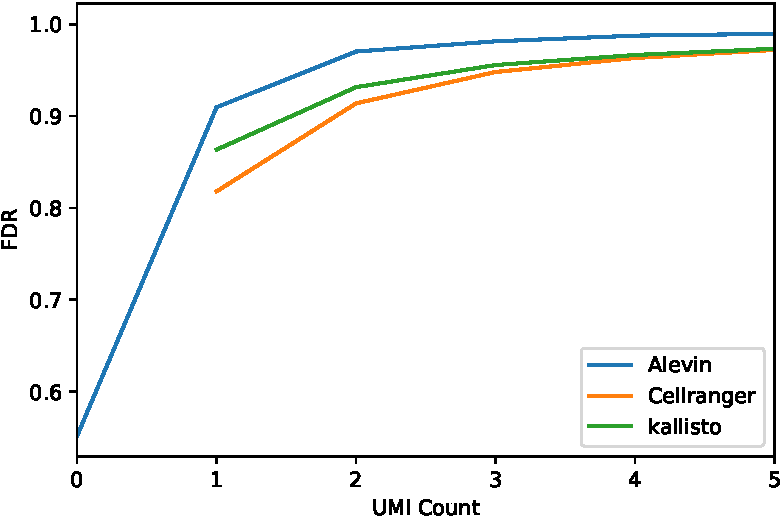
\includegraphics[width=\linewidth]{alevin2/fdr.pdf}
    \caption{ Comparison of False Discovery Rate (FDR) i.e. including both FP and FN with the
	the number of mispredicted UMIs. }
    \label{fig:alv2_fdr}
  \end{figure}

  \begin{figure}[!htb]
      \centering
    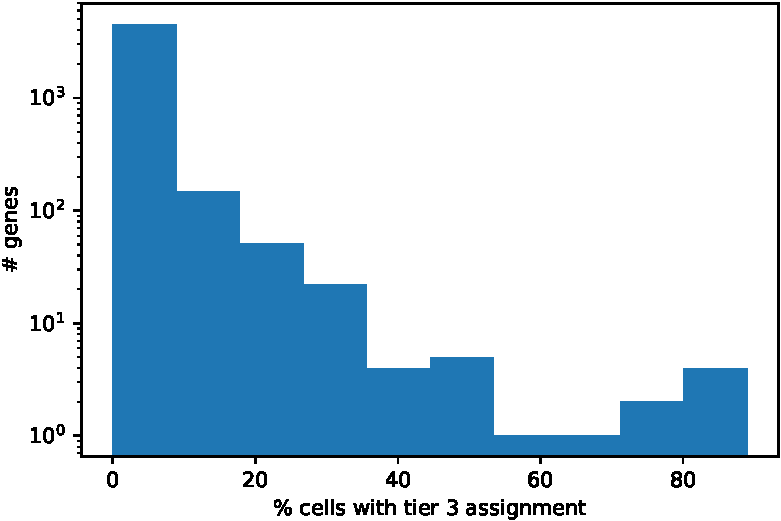
\includegraphics[width=\linewidth]{alevin2/t3_assign.pdf}
    \caption{ The distribution of the number of genes with the fraction of cells they have tier3
	assignment.}
    \label{fig:alv2_t3}
  \end{figure}

In ~\Cref{fig:alv2_fdr} we show the fraction of false discoveries which are covered by the
extent in a method's mis-estimation. We include both FP and FN as false discoveries and 
find that more than 90\% of alevin's false predictions are below 1 UMI count. 

\subsection{Variational Bayesian Improves dscRNA-seq quantification}
In ~\Cref{alevin}, we categorize the confidence in the generated gene counts estimates using tiers. 
Even though ~\Cref{subsec:alv2_sims}, we show the alevin generated quants are more accurate
than competing tools, the confidence in tier3 assigned estimates is low and often the source of 
the mis-estimation. We found that in the simulated data, more than 66\% of the false discoveries made 
by alevin are in the tier3 estimates and due to the inherant problem of sparsity in dscRNA-seq data,
we expect the similar pattern of tier3 genes in the real data as well. 

In \Cref{fig:alv2_t3} we show the distribution of the genes with tier3 prediction in at least one cell,
versus the percentage of cells they have tier3 prediction overall. This aligns with the fundamental 
property of a dscRNA-seq experiments i.e. molecules are randomly captured across cells and although
some cells might randomly sample the read sequence from the ambiguous region (or no sample at all) but, 
in expectation, similar cells in a group can potentially have different confidence in their gene
estimation. Hence, to improve the expression estimates of the tier3 genes, we proposed the idea of 
information sharing across cells (details in ~\Cref{sec:alv2_methods}).

\subsubsection{Migration Experiment onf Real Data}


\section{Conclusion}
We proposed a bayesian framework which extends previous generation alevin's maximum likelihood based 
quantification procedure. We explore different techniques of generating priors and show that our 
information sharing framework consistently improves the tier3 dscRNA-seq quantification estimates and 
is especially useful for highly ambiguous estimates where there is no intra cellular activity to 
effiiently quantify. We plan to extend the framework towards incorporating priors from new upcoming 
technologies, for example spatial data can be substantially useful for setting the prior in the proposed 
alevin framework.  We think this framework has potential to open a new direction of multi-modal 
quantification of the data and the community will adopt and help improve it further.
